\documentclass[doubleblind]{elsarticle}\usepackage[]{graphicx}\usepackage[]{color}
% maxwidth is the original width if it is less than linewidth
% otherwise use linewidth (to make sure the graphics do not exceed the margin)
\makeatletter
\def\maxwidth{ %
  \ifdim\Gin@nat@width>\linewidth
    \linewidth
  \else
    \Gin@nat@width
  \fi
}
\makeatother

\definecolor{fgcolor}{rgb}{0.345, 0.345, 0.345}
\newcommand{\hlnum}[1]{\textcolor[rgb]{0.686,0.059,0.569}{#1}}%
\newcommand{\hlstr}[1]{\textcolor[rgb]{0.192,0.494,0.8}{#1}}%
\newcommand{\hlcom}[1]{\textcolor[rgb]{0.678,0.584,0.686}{\textit{#1}}}%
\newcommand{\hlopt}[1]{\textcolor[rgb]{0,0,0}{#1}}%
\newcommand{\hlstd}[1]{\textcolor[rgb]{0.345,0.345,0.345}{#1}}%
\newcommand{\hlkwa}[1]{\textcolor[rgb]{0.161,0.373,0.58}{\textbf{#1}}}%
\newcommand{\hlkwb}[1]{\textcolor[rgb]{0.69,0.353,0.396}{#1}}%
\newcommand{\hlkwc}[1]{\textcolor[rgb]{0.333,0.667,0.333}{#1}}%
\newcommand{\hlkwd}[1]{\textcolor[rgb]{0.737,0.353,0.396}{\textbf{#1}}}%
\let\hlipl\hlkwb

\usepackage{framed}
\makeatletter
\newenvironment{kframe}{%
 \def\at@end@of@kframe{}%
 \ifinner\ifhmode%
  \def\at@end@of@kframe{\end{minipage}}%
  \begin{minipage}{\columnwidth}%
 \fi\fi%
 \def\FrameCommand##1{\hskip\@totalleftmargin \hskip-\fboxsep
 \colorbox{shadecolor}{##1}\hskip-\fboxsep
     % There is no \\@totalrightmargin, so:
     \hskip-\linewidth \hskip-\@totalleftmargin \hskip\columnwidth}%
 \MakeFramed {\advance\hsize-\width
   \@totalleftmargin\z@ \linewidth\hsize
   \@setminipage}}%
 {\par\unskip\endMakeFramed%
 \at@end@of@kframe}
\makeatother

\definecolor{shadecolor}{rgb}{.97, .97, .97}
\definecolor{messagecolor}{rgb}{0, 0, 0}
\definecolor{warningcolor}{rgb}{1, 0, 1}
\definecolor{errorcolor}{rgb}{1, 0, 0}
\newenvironment{knitrout}{}{} % an empty environment to be redefined in TeX

\usepackage{alltt}

\usepackage{lineno,hyperref}
\modulolinenumbers[5]

\usepackage{amsmath,amsthm}
\usepackage{graphicx,psfrag,epsf}
\usepackage{enumerate}
\usepackage{booktabs}
\usepackage{longtable}
\usepackage{array}
\usepackage{multirow}
\usepackage{adjustbox}
\usepackage[table]{xcolor}
\usepackage{wrapfig}
\usepackage{subfig}
\usepackage{float}
% \usepackage{colortbl}
\usepackage{pdflscape}
\usepackage{tabu}
\usepackage{threeparttable}

\usepackage[numbers]{natbib}

\newenvironment{definition}[1]% environment name 
{% begin code 
  \par\vspace{.75\baselineskip}\noindent 
  \textbf{Definition (#1)}\begin{itshape}% 
  \par\vspace{.5\baselineskip}\noindent\ignorespaces 
}% 
{% end code 
  \end{itshape}\ignorespacesafterend 
}

\providecommand{\tightlist}{%
  \setlength{\itemsep}{0pt}\setlength{\parskip}{0pt}}


\journal{Forensic Science International}
%%%%%%%%%%%%%%%%%%%%%%%
%% Elsevier bibliography styles
%%%%%%%%%%%%%%%%%%%%%%%
%% To change the style, put a % in front of the second line of the current style and
%% remove the % from the second line of the style you would like to use.
%%%%%%%%%%%%%%%%%%%%%%%

%% Numbered
%\bibliographystyle{model1-num-names}

%% Numbered without titles
%\bibliographystyle{model1a-num-names}

%% Harvard
% \bibliographystyle{model2-names.bst}\biboptions{authoryear}

%% Vancouver numbered
%\usepackage{numcompress}\bibliographystyle{model3-num-names}

%% Vancouver name/year
%\usepackage{numcompress}\bibliographystyle{model4-names}\biboptions{authoryear}

%% APA style
% \bibliographystyle{model5-names}\biboptions{authoryear}

%% AMA style
%\usepackage{numcompress}\bibliographystyle{model6-num-names}

%% `Elsevier LaTeX' style
\bibliographystyle{elsarticle-num-names}
%%%%%%%%%%%%%%%%%%%%%%%
\IfFileExists{upquote.sty}{\usepackage{upquote}}{}
\begin{document}

\begin{frontmatter}

\title{Comparison of three similarity scores for bullet LEA matching\tnoteref{t1}\tnoteref{t2}}

\tnotetext[t1]{This work was partially funded by the Center for Statistics and Applications in Forensic Evidence (CSAFE) through Cooperative Agreement \#70NANB15H176 between NIST and Iowa State University, which includes activities carried out at Carnegie Mellon University, University of California Irvine, and University of Virginia.}

\tnotetext[t2]{The authors wish to thank Alan Zheng (NIST), Tylor Klep (Phoenix PD), and Melissa Nally and Kasi Kirksey (FSI Houston) for access to test set bullets. We would also like to thank the efforts of the Roy J Carver High Resolution lab in scanning the bullet sets and providing the scans to us.}

%% Group authors per affiliation:
% \author{Elsevier\fnref{myfootnote}}
% \address{Radarweg 29, Amsterdam}
% \fntext[myfootnote]{Since 1880.}

%% or include affiliations in footnotes:
% \author[mymainaddress,mysecondaryaddress]{Elsevier Inc}
% \ead[url]{www.elsevier.com}
% 
% \author[mysecondaryaddress]{Global Customer Service\corref{mycorrespondingauthor}}
% \cortext[mycorrespondingauthor]{Corresponding author}
% \ead{support@elsevier.com}
% 
% \address[mymainaddress]{1600 John F Kennedy Boulevard, Philadelphia}
% \address[mysecondaryaddress]{360 Park Avenue South, New York}

\author[isu,csafe]{Heike Hofmann}
\cortext[corauthor]{Corresponding author}\ead{srvander@iastate.edu}
\author[isu,csafe]{Susan Vanderplas\corref{corauthor}}
\address[isu]{Statistics Department, Iowa State University\\2438 Osborne Dr, Ames, IA 50011}
\address[csafe]{Center for Statistical Applications in Forensic Evidence, Iowa State University\\613 Morrill Rd, Ames, IA 50011}
   

\begin{abstract}
Recent advances in microscopy have made it possible to collect 3D topographic data, enabling more precise virtual comparisons based on the collected 3D data as a supplement to traditional comparison microscopy and 2D photography. Automatic comparison algorithms have been introduced for various scenarios, such as matching cartridge cases \citep{tai2018fully,song3DTopographyMeasurements2014} or matching bullet striae \citep{aoas2, chuAutomaticIdentificationBullet2013, dekinderAutomatedComparisonsBullet1999}. One key aspect of validating these automatic comparison algorithms is to evaluate the performance of the algorithm on external tests, that is, using data which were not used to train the algorithm. Here, we present a discussion of the performance of the matching algorithm \citep{aoas2} in three studies conducted using different Ruger weapons. We consider the performance of three scoring measures: random forest score, cross correlation, and consecutive matching striae (CMS) at the land-to-land level and, using Sequential Average Maxima scores, also at the bullet-to bullet level. Cross correlation and random forest scores both result in perfect discrimination of same-source and different-source bullets. At the land-to-land level, discrimination for both cross correlation and random forest scores (based on area under the curve, AUC) is excellent ($\ge$ 0.90).
\end{abstract}

\begin{keyword}
forensic science, toolmark, cross correlation, random forest, 3D microscopy, land engraved areas (LEAs)
\end{keyword}

\end{frontmatter}



\newcommand{\hh}[1]{{\textcolor{orange}{#1}}}
\newcommand{\svp}[1]{{\textcolor{teal}{#1}}}
\noindent

% \hh{
% Cleanup TO-DO
% \begin{itemize}
% \item \sout{define false positives and false negatives once and stick to those definitions. We should avoid false positive and false negatives, because that only makes sense in a test setting, which we have not defined formally.
% Let's use instead wrong identification and missed identification. }
% \item \sout{error rates: we are using rates exchangeably with percentages. We need to fix that. I think percentages might be easier understood. XXX Should be fixed now}
% \end{itemize}
% }
% \svp{
% Outstanding XXX items:
% \begin{itemize}
% \item ``Authors are responsible for obtaining written permission from persons acknowledged by name, because readers may infer their endorsement of the data and conclusions."
% \item thanks - scanning and hamby advice
% \item comparison to FTEs in conclusion
% \end{itemize}
% }





 
In current practice, firearms and toolmark examiners (FTE) evaluate the similarity of striae on bullets by placing the evidence together with another bullet under a comparison microscope. The second bullet could be a test fire from a weapon recovered during the investigation, or it could be a second bullet from the crime scene. Examiners visually classify similarity according to the theory of firearms identification \citep{identification} as one of identification, inconclusive or exclusion. Exact guidelines for this classification vary from lab to lab; some labs will exclude only on the basis of non-matching class characteristics, such as direction of the twist in rifling, land length or number of lands, or type of rifling. In other labs, CMS (consecutively matching striae) as defined by \citeauthor{biasotti} \citep{biasotti} is used as a measure to quantify the similarity of two lands. In virtually all labs, individual characteristics used to identify matching bullets are derived from visual assessment; some class characteristics may be directly measured, but these are not sufficient for individualization. 

% Identification using 3D Scanning Technology

More explicit characterization of bullet surfaces has been discussed since at least 1958 by \citeauthor{davis1968introduction} \cite{davis1968introduction}, but at the time technology was not sufficiently advanced to make an analysis based on 3D measurements or surface traces a viable option. \citet{ComputerIdentificationBullets1978} demonstrated use of a scanning electron microscope to quantitatively examine and compare bullet striae. More recently, approaches using 3D measurement data were explicitly described in 1999 by \citeauthor{dekinderAutomatedComparisonsBullet1999} \cite{dekinderAutomatedComparisonsBullet1999}, and have been further developed in \citep{bachrachDevelopment3DbasedAutomated2002,xieAutomatedBulletidentificationSystem2009, chuPilotStudyAutomated2010}. These approaches utilize 3D surface measurements directly to characterize the topology of land engraved areas (LEAs), rather than using visual or image comparison techniques. In many cases, these approaches also provide some level of automation of the comparison process, with the goal of reducing human biases by augmenting the visual information with 3D measurements. Utilizing the 3D measurements allows for examination of both peaks and valleys in LEAs. It also allows us to take the depth of striae into account; something that is difficult, if not impossible, from visual inspection.

Commonly, approaches derived from 3D surface measurements use some features which are similar to those visually assessed by FTEs \citep{luAutomatedBulletIdentification2014}. Class characteristics, which are shared by a group of firearms with the same rifling design, manufacturer, and tooling process, are typically evaluated first, as a mismatch on class charcteristics is sufficient for an exclusion. Automated approaches to estimation of width of the land engraved area and twist angle were described in \citet{chuPilotStudyAutomated2010}. Individual characteristics, which are not shared by all members of a class, can also be automatically assessed from 3D surface measurements. One of the most common features used to describe the similarity of two surfaces is the cross correlation function, which is utilized in several studies \citep{maNISTBulletSignature2004, vorburgerApplicationsCrosscorrelationFunctions2011, chuPilotStudyAutomated2010}. Additional features proposed for automatically assessing similarity also include signature distance \citep{maNISTBulletSignature2004}, striae depth and width \citep{ComputerIdentificationBullets1978}, and consecutive matching striae (CMS) \citep{chuAutomaticIdentificationBullet2013}.

\section{Methods}

In the matching algorithm proposed in \citet{aoas2}, several features are combined using a random forest \citep{breiman} to produce a similarity score based on 3D topographic scans of land engraved areas (LEAs). In order to generate these features, some pre-processing is necessary in order to transform the 3D surface measurements into `signatures' which can be compared.

\subsection{Automated Processing of 3D Scans}

From each land engraved area a signature is derived using the process described in detail in \citet{aoas2}:

\begin{itemize}
\item[(a)] Identify an area on the LEA with expressed striae. Locate a stable crosscut in the identified area; that is, an area where the striae are similar in the region above and below the crosscut. This excludes regions with extreme pitting, breakoff, tank rash, and other flaws that would interfere with similarity score calculation.
\item[(b)] Discard extraneous/contaminated data, such as data from groove engraved area and areas affected by break-off or contact with objects after the bullet exited the barrel  (``tank rash").
\item[(c)] Remove bullet curvature using a non-parametric smooth. 
\end{itemize}
A signature for a land engraved area is then defined as the sequence $S(x)$, $x = 1, ..., I$, where $I$ is the number of observed locations across the base of the bullet. \autoref{fig:signatures} shows a set of six signatures corresponding to the six land engraved areas of bullets 1 and 2 from barrel 1 of set 44 of the Hamby study \citep{hamby}. 
\begin{knitrout}
\definecolor{shadecolor}{rgb}{0.969, 0.969, 0.969}\color{fgcolor}\begin{figure}

{\centering \includegraphics[width=\textwidth]{figures/signatures-1} 

}

\caption[Signatures of all six lands of bullets 1 and 2 from barrel 1 of the Hamby set 44]{Signatures of all six lands of bullets 1 and 2 from barrel 1 of the Hamby set 44. Matching lands between the two bullets have been placed above each other.}\label{fig:signatures}
\end{figure}


\end{knitrout}

Once signatures have been extracted from stable regions with expressed striae, they must be aligned in order to assess their similarity, just as examiners would manually align two bullets under a comparison microscope. Maximized cross correlation is used to pair-wise align signatures \citep{aoas2,vorburgerApplicationsCrosscorrelationFunctions2011}. 

The cross correlation (CC) function between two signatures $S_1(x)$ and $S_2(x)$ is defined as 
\[
CC(S_1, S_2, z) = \text{cor}\left(S_1(x), S_2(x + z)\right)
\] 
where $x$ and $x+z$ are integer values appropriately defined within the domains of $S_1$ and $S_2$, $z$ is the lag between the two sequences, and $\text{cor}(.,.)$ is the Pearson correlation coefficient.
When signatures contain missing values, pairwise complete observations are used to calculate the cross correlation. The lag $z$ used to achieve maximum $CC$ is used to determine the best alignment.


\subsection{Statistics for Matching Aligned Signatures}

Using the lag determined for aligning two signatures, other quantitative features describing the similarity of the two signatures can be extracted. Numerical features such as cross correlation and Euclidean distance can be computed from the aligned signatures alone. Additional features are modeled after visual assessment methods used by examiners, including striae depth, total number of matching striae, and the number of consecutively matching striae (CMS).

In order to evaluate CMS, we must first identify peaks and valleys in each of the signatures, then determine whether these peaks and valleys overlap sufficiently. Features which firearms examiners assess visually generally depend on the identification of these extrema, as striation marks and the corresponding peaks are the most salient feature when viewing a bullet using a microscope. If there are at least six consecutive matching striae, the bullets are considered to be similar in practice \citep{biasotti_firearms_1997,nichols_scientific_2006}. CMS, as measured by examiners, is the number of consecutively matching peaks in signatures of two aligned lands, and, because examiner typically lines up two distinctive markings, resulting in at least one matching striation mark. Peaks -- rather than peaks and valleys -- are used in part because it is difficult to visually assess valleys except as relative to peaks. In contrast, the matching algorithm can identify both peaks and valleys, and signatures are aligned based on maximum cross-correlation (as opposed to matching striation marks), there is the possibility that two lands will have zero consecutive matching striae. Thus, the matching algorithm uses a slightly different measure of CMS than examiners, but the underlying principle is the same. The algorithms used to identify peaks and valleys in each signature and determine CMS from the peak and valley identifications are described in more detail in \citep[p. 2340, step 3 -- 4]{aoas2}. 

% <!-- I really think this belongs in this section: it's discussing cross correlation as a scoring statistic, rather than as a convenient way to align signatures so that scoring stats can be calculated. --> 

Cross correlation can also be used to assess similarity between two aligned signatures. Cross correlation varies between -1 and 1, but as the alignment is based on the maximized cross correlation value, in practice the cross correlations for aligned signatures are generally positive. Cross correlation values which are close to 1 indicate similarity between signatures, with the possibility that the two signatures come from the same source. Low cross correlation values indicate signatures which are different and thus may originate from different sources.

The random forest presented in \citet{aoas} is based on a combination of multiple characteristics, including cross correlation, number of matching striae, and number of consecutively matching striae. The output of the random forest is a score between 0 and 1 representing the algorithm's assessment of the similarity of the two signatures, where scores close to 1 indicate signatures which are similar and may have originated from the same source, while scores close to 0 indicate that the aligned signatures are different and may originate from different sources.

\subsection{Interpreting the Algorithm Score}

The features described above are each individually designed to separate same-source and different-source signatures: for instance, same-source signatures would have high cross correlation values and different-source signatures would have low cross correlation values. For each feature, or an aggregate score composed of many features, the end result for any two signatures is a number which must be compared to a distribution of other scores from similar situations.

Using this distribution of scores and training data, an automated algorithm selects a cutoff value, introducing a barrier between identification and exclusion. This threshold system introduces a binary classification: identification or exclusion. This definition of error is more stringent than the AFTE Theory of Identification, in that it does not allow for inconclusive results. This increased rigor may increase the error rate of the model when compared to examiner error rates, but we expect that the increased information available from the 3D measurement data will compensate for this loss. A binary decision model is also easier to interpret and provides more clear-cut, definitive results than the AFTE Theory of Identification system used in most forensic laboratories in the United States. Of course, in jurisdictions which utilize score-based likelihood ratios, this threshold system is not necessary because likelihood ratios are continuous. Even with likelihood ratios, however, there is a natural threshold at 1 which functions similarly to the selected threshold in the binary decision case. 

The remainder of this paper will utilize the binary decision model which is compatible with the legal framework commonly used in US jurisdictions. With this model, we can enumerate characteristics of an ideal similarity scoring mechanism: 

\begin{description}
\item[(R1)] {\bf Monotonicity:} a higher score is indicative of higher similarity between a pair of bullets, in particular, similarity scores of same-source pairs of bullets are higher than different-source pairs.
\item[(R2)] {\bf Stability:} the same score leads to the same conclusion in all situations and under separately assembled reference distributions. 
\end{description}

In particular, requirement (R2) would imply that the same threshold value would be used for all comparisons of a certain scoring mechanism. If the same-source and different-source similarity score distributions overlap, setting a threshold value will introduce classification errors.


\subsection{Identification Errors and Algorithm Evaluation}

When evaluating algorithm performance, it is useful to systematically assess  the set of possible outcomes. If ground truth and the algorithm's prediction match, we have either a correct identification or a correct exclusion. If ground truth and the algorithm's prediction do not match, we distinguish between two types of errors, which we will refer to as \textbf{wrong identification} and \textbf{missed identification}. Wrong identifications are those in which two bullets from different sources are determined to be from the same source. Missed identifications are those in which two bullets from the same source are determined to be from different sources. The full range of possible outcomes is shown in \autoref{tab:possible-outcomes}.

\begin{table}
\centering
\bgroup
\def\arraystretch{.8}%  1 is the default, change whatever you need
\begin{tabular}{|ccc}
\multicolumn{1}{c}{} & \multicolumn{2}{c}{\textbf{Ground Truth}}\\\cline{2-3}
\multicolumn{1}{c}{\textbf{Results}} & \multicolumn{1}{|c}{Same Source} & \multicolumn{1}{|c|}{Different Source} \\\hline
\multirow{2}{*}{Exclusion} & \multicolumn{1}{|c}{Missed} & \multicolumn{1}{|c|}{Correct}\\
   &  \multicolumn{1}{|c}{Identification} & \multicolumn{1}{|c|}{Exclusion}\\\hline
\multirow{2}{*}{Identification}  &  \multicolumn{1}{|c}{Correct} & \multicolumn{1}{|c|}{Wrong}\\
   &  \multicolumn{1}{|c}{Identification} & \multicolumn{1}{|c|}{Identification}\\\hline
\end{tabular}
\egroup
\caption{Possible outcomes of an examination of two pieces of evidence. Correct decisions are shown in the top-right and bottom-left corners; incorrect decisions in the top-left and bottom-right corners.\label{tab:possible-outcomes}}
\end{table}


In machine learning and statistics, it is common to evaluate algorithms using sensitivity and specificity; these concepts are related to the error rate. \textbf{Sensitivity} is defined as the proportion of actual positives that are correctly identified; that is, when ground truth is same source, the sensitivity is the proportion of correct identifications. \textbf{Specificity} is defined as the proportion of actual negatives that are correctly identified; that is, when ground truth is different source, the specificity is the proportion of correct identifications. The combination of sensitivity and specificity is sufficient to describe the reliability of an algorithm. 

When evaluating the \citet{aoas2} algorithm, we will describe errors as a percentage of correct evaluations. Statistics that do not translate to percent-form interpretation, such as area under the curve (AUC), will be presented as a decimal. 

\subsection{Assessing Bullet-to-Bullet Similarity}

Each of the scoring methods we have described is computed on a land-to-land basis. While these comparisons are useful, the question of interest typically involves the entire physical object (e.g. all lands on a single bullet), and a conclusion on same or different source should be reached based on the evidence of all lands of the two bullets.



Land-to-land comparisons lead to a whole set of scores to evaluate for bullet-to-bullet comparisons. \autoref{fig:b2b} shows two matrices of scores for two pairs of bullet-to-bullet matches. On the left, a matrix is shown that is typical for scores from two bullets from the same barrel. On the right, values for a pair of known non-matching bullets are shown.


\begin{knitrout}
\definecolor{shadecolor}{rgb}{0.969, 0.969, 0.969}\color{fgcolor}\begin{figure}

{\centering \includegraphics[width=.6\textwidth]{figures/b2b-1} 

}

\caption[Overview of land-land matching scores for two pairs of bullet-bullet comparisons]{Overview of land-land matching scores for two pairs of bullet-bullet comparisons. On the left the two bullets are known to come from the same source (barrel) on the right, the bullets are from two different sources (barrels).}\label{fig:b2b}
\end{figure}


\end{knitrout}

While some imaging systems, such as BulletTrax 3D\footnote{https://www.ultra-forensictechnology.com/en/our-products/ballistic-identification/bullettrax/} or BalScan\footnote{https://www.forensic.cz/en/products/balscan}, may capture lower-resolution scans of an entire bullet at one time, confocal light microscopes do not have 360$^\circ$ capability. Thus, when imaging bullets using a confocal light microscope, operators scan one land at a time in a clockwise (left twisted rifling) or anti-clockwise (right twisted rifling) sequence. The order in which scans are acquired is kept as meta-information. 

Let us assume that lands on a bullet are labelled $\ell_i$ with $i = 1, .., p$, where $p$ indicates the number of lands a bullet has, as determined by the rifling of a barrel. For all of the bullets considered here the number of lands, $p$, is 6. A match between  a pair of lands from two bullets therefore results in an expected additional $p-1$ matches between pairs of lands. These lands are also expected to be in a sequence, i.e. if there is a match between lands $\ell_i$ on bullet 1 and $\ell_j$ on bullet 2, we also expect lands $\ell_{i\oplus s}$ and $\ell_{j\oplus s}$ to match for all integers $s$, where $\oplus$ is defined as $a \oplus b \equiv \left((a + b - 1)\mod p\right) + 1$. This relationship gives rise to the sequence average maximum (SAM) to quantify a bullet-to-bullet match. 

\begin{definition}{Sequence Average and its Maximum}
Let $A$ be a square real-valued matrix of dimensions $p \times p$. For the purpose of this paper, $A$ consists of scores describing the similarity between two sets of land engraved areas. The entries in $A$ are represented as $a_{i,j}$, where $i$ and $j$ are row and column indexes. 

The $k$th \emph{sequence average} $SA(A, k)$ for $k = 0, ... p-1$ is defined  as 
$$SA(A, k) = \frac{1}{p} \sum_{i=1}^{p} a_{i,i \oplus k}, \text{ where } i\oplus k := \left((i + k - 1)\mod p\right) + 1.$$
The \emph{Sequence Average Maximum} \citep[SAM, ][]{sam} of square matrix $A$ of scores is defined as
$$SAM (A) = \max_{k = 1}^{p} SA(A, k).$$
\end{definition}
Looking back at \autoref{fig:b2b}, we see that for the two bullets from the same barrel, the sequence average for 
$k=2$ is higher than the other sequence averages, and also higher than the sequence averages for the other pair of bullets shown on the right of the figure. SAM scores allow us to define a single quantity for each pair of bullets that describes the similarity between these two bullets. 

The sequence average maximum of the correlation between lands is used in SensoComp \citep{sensofar-sam} to capture the similarity between bullets. The correlation based SAM score has also been called the 'average correlation calculated at the max phase' in \citet{chuPilotStudyAutomated2010}. 

\begin{knitrout}
\definecolor{shadecolor}{rgb}{0.969, 0.969, 0.969}\color{fgcolor}\begin{figure}

{\centering \includegraphics[width=\textwidth]{figures/sam-sketch-1} 

}

\caption[Sketch of all six land-to-land sequences between two bullets with six lands]{Sketch of all six land-to-land sequences between two bullets with six lands.}\label{fig:sam-sketch}
\end{figure}


\end{knitrout}


Random forests \citep{breiman} have a built-in internal testing mechanism to prevent potential overfitting. Errors reported by random forest algorithms are based on these internal test sets, though there is some debate about the bias of these errors \citep{rfOver2, rfOver}. 
Neither of these papers addresses another issue with internal test sets: internal test sets are constructed to have the same distribution as the training data (apart from sampling variability). For any machine learning method, a true benchmark of the performance of an algorithm requires testing its performance on external test data. Good performance (in terms of wrong and missed identifications) on external test data validates a ML algorithm. External data also allows an assessment of the algorithm's sensitivity to distributional changes as well as testing the algorithm's robustness by going outside the parameters of the training data.  

In this paper, we validate the algorithm described in \citet{aoas2} on three external test sets. We assess the results on each set and evaluate whether the minimal requirements described above are fulfilled for bullet-to-bullet SAM scores. We compare the random forest algorithm's performance to the performance of other suggested measures for quantitative assessment of bullet similarity, such as cross correlation and consecutive matching striae. 

\section{Validation Sets}

The algorithm in \citet{aoas2} is trained on scans from Hamby sets 252 and 173 made available through \citet{nist}. Set 173 was originally published as Hamby set 44, but the mis-labeling has been recently corrected. The scans used to train the model were taken at 20 fold magnification for a resolution of 1.5625 microns per pixel. While magnification is generally of interest in microscopy, \emph{resolution} -- usually measured in microns per pixel -- is of more interest for 3D topographic measurements, as it determines the operative level of available data.

For the validation of the automatic matching algorithm we are considering three validation sets of -- what should be -- increasing difficulty level: 
\begin{itemize}
\item {\bf Hamby set 44} is one set of the Hamby study \citep{hamby}. Each Hamby set  consists of a total of 35 bullets fired through ten consecutively manufactured barrels of Rugers P85. Each set consists of 20 known bullets (two from each of the ten barrels) and 15 questioned bullets of unknown origin. Note that all Hamby sets are closed sets; that is, all questioned bullets are fired through one of the ten barrels. The ammunition used for this set were 9 mm Luger 115 Grain Full Metal Jacket  from the Winchester Ammunition Company.
\item {\bf Phoenix PD}
Tylor Klep from Phoenix PD provided sets of known test fires and questioned bullets: the set of known bullets consists of three test fires (B1, B2, B3) from each of eight different, consecutively rifled Ruger P-95 barrels (A9, C8, F6, L5, M2, P7, R3, U10). Ten questioned bullets were provided (B, E, H, J, K N, Q, T, Y, Z). This set is an open set; that is, it is not known in advance whether all (or any) of the questioned bullets are fired from the known barrels. In fact, the results will show that three of the questioned bullets were fired from three different barrels not included in the knowns. These three barrels correspond to an eleventh Ruger P-95 barrel, a Ruger P-95C barrel and a Ruger P-85 barrel. All bullets fired for this study are American Eagle 9mm  Luger full metal jackets.
Land engraved areas for each of the six lands of each bullet were scanned by Bill Henderson (Sensofar).
\item {\bf Houston FSI}
This study was set up by Melissa Nally and Kasi Kirksey from FSI Houston. Three test sets based on ten consecutively rifled Ruger LCP barrels (A, B, C, D, E, F, G, H, I, J) and three other, non-consecutively rifled Ruger LCP barrels (R1, R2, R3). Each test set consists of three test fires each from five consecutively rifled barrels. Additionally, ten questioned bullets are provided for each kit. The ammunition used in both test fires and the questioned bullets were Remington UMC 9mm Luger Full Metal Jackets. All three of the test sets are open; that is, not every one of the questioned bullets is fired from the five known barrels in each of the test set.
The structure of these three sets is similar to a forthcoming study by Nally and Kirksey, but the results here come from preliminary test sets made available to us.
\end{itemize}
 
Scans of all land engraved areas for the validation data were taken on a Sensofar Confocal Light microscope at 20x magnification resulting in a resolution of 0.645 microns per pixel. If not indicated otherwise, scans were taken at the Roy J Carver high resolution microscopy lab at Iowa State University.
 
Case studies were chosen such that theoretical difficulty for the matching algorithm increases with each case study: Hamby set 44 is part of the Hamby study. The algorithm in \citet{aoas2} was trained on sets 173 and 252, so the bullets in Hamby 44 are of the same type of ammunition and are fired through the same barrels as the bullets in the training set. The Phoenix PD set uses Ruger P-95 barrels, which are different from the barrels in the Hamby sets used for training the algorithm, but the barrels are rifled similarly to the Ruger P-85 barrels. The Houston sets use Ruger LCP barrels. These barrels are first rifled traditionally, i.e. similar to the Ruger P-85, but are treated with a secondary round of heating after rifling, which may introduce some subclass characteristics. This should make the automatic matching harder, and in particular, is expected to complicate the classification as different-source land engraved areas/bullets. In all three studies, the scan resolution is much higher than the scans used to train the algorithm in \citet{aoas2}; this difference also provides a test of the algorithm's ability to generalize to scans taken at different resolutions.

\section{Results}

\subsection{Hamby Set 44}

\begin{knitrout}
\definecolor{shadecolor}{rgb}{0.969, 0.969, 0.969}\color{fgcolor}\begin{figure}

{\centering \includegraphics[width=\textwidth]{figures/h44-1} 

}

\caption[Hamby set 44]{Hamby set 44: overview of all bullet-to-bullet matches between all pairs of questioned bullets (y-axis) and known test fires from ten barrels (x axis).}\label{fig:h44}
\end{figure}


\end{knitrout}

\autoref{fig:h44} shows an overview of all scores from pairs of questioned bullets with all other bullets. On the left of \autoref{fig:h44} there are ten strips labelled 1 through 10. These strips correspond to known barrels 1 through 10. Each barrel was test-fired twice, so each of the questioned bullets (shown along the $y$ axis) matches two bullets fired from a known barrel. Colored tiles are used to show the similarity score: light grey colors correspond to low similarity scores, dark colors correspond to high similarity scores. Ground truth is encoded in this figure as a thin, dark, colored frame for all pairs of same-source bullets. 
Ideally, we want to see one barrel with two dark-filled, dark-framed tiles for each questioned bullet, and light grey tiles for all other barrels, indicating a match between a questioned bullet and a single barrel. This expectation is met for all questioned bullets, i.e.\ the automatic matching  identifies the correct barrel for all questioned bullets. For two of the questioned bullets, 'I' and 'F', the similarity scores to the matching barrels are considerably smaller than for the other questioned bullets. 

The right side of \autoref{fig:h44} shows the relationship between all pairs of questioned bullets. Note that questioned bullets are not compared to themselves, leaving white squares on the diagonal. Some of the questioned bullets match the same barrel, e.g.\ questioned bullets 'P' and 'J' both match barrel 5. Therefore bullets 'P' and 'J' also match each other in the square on the right hand side.



\subsection{Phoenix PD}

\begin{knitrout}
\definecolor{shadecolor}{rgb}{0.969, 0.969, 0.969}\color{fgcolor}\begin{figure}

{\centering \includegraphics[width=\textwidth]{figures/pd-1} 

}

\caption[Phoenix study]{Phoenix study: overview of all bullet-to-bullet matches between all pairs of questioned bullets (y-axis) and known test fires from ten barrels (x axis). The order of the bullets on the y axis is determined by matching barrel.}\label{fig:pd}
\end{figure}


\end{knitrout}

\autoref{fig:pd} shows an overview of similarity scores for all pairs of questioned bullets and  test fires. The color encoding is the same as in the previous figures. Here, we see that questioned bullets either match all 3 bullets fired out of the same barrel for exactly one of the barrels or none of the known barrels. Questioned bullets 'Q', 'Y', and 'Z', do not match any of the known barrels.
None of the test fires from barrel U10 match any of the questioned bullets.  This is a sign of the previously mentioned open set characteristic of the study. 
Once again, the results from automatic matching correctly pair questioned bullets with their corresponding barrels.

\subsection{Houston FSI}

\autoref{fig:hou} shows an overview of the three sets of scores for all pairs of questioned bullets with all other bullets in the set. In set 1, five of the questioned bullets can be matched to known bullets in the set. None of the questioned bullets in set 1 match bullets fired from barrels KC or KD. Additionally, two of the questioned bullets which do not match any of the barrels in the set match each other (U28 and U37). In set 2, four of the questioned bullets can be matched to known bullets in the set; of the additional four questioned bullets which do not match any known bullets, two were fired from the same barrel (bullets U34 and U73). In set 3, six of the questioned bullets match known bullets, and the remaining two questioned bullets match each other (bullets U14 and U45) but do not match any known bullets in the set. 
% <!--Thus, we can conclude that the algorithm performs well on open set studies, as it can identify matches among questioned bullets which do not match any known bullets. -->
While all bullet-to-bullet matches are correctly identified, and no known matches are missed, it is obvious from the generally lighter shades of the tiles corresponding to matching bullets in \autoref{fig:hou}(b) that the algorithm is not performing as well on set 2 as it performs on sets 1 and 3.

\begin{knitrout}
\definecolor{shadecolor}{rgb}{0.969, 0.969, 0.969}\color{fgcolor}\begin{figure}
\subfloat[Set 1\label{fig:hou1}]{\includegraphics[width=\textwidth]{figures/hou-1} }\newline
\subfloat[Set 2\label{fig:hou2}]{\includegraphics[width=\textwidth]{figures/hou-2} }\newline
\subfloat[Set 3\label{fig:hou3}]{\includegraphics[width=\textwidth]{figures/hou-3} }\caption[Overview of matching scores for all pairs of questioned bullets to known bullets from five barrels (on the left) and questioned bullets to themselves (tiles on the right)]{Overview of matching scores for all pairs of questioned bullets to known bullets from five barrels (on the left) and questioned bullets to themselves (tiles on the right).}\label{fig:hou}
\end{figure}


\end{knitrout}


\section{Evaluating the Random Forest Algorithm}
The random forest scores correctly separate known matches from known non-matches, using SAM scores to aggregate land-to-land scores into a bullet-to-bullet comparison. With no errors at the bullet-to-bullet level, we can now evaluate the scores in light of (R1) and (R2). In this section, we will primarily compare the random forest scores to cross correlation scores; cross correlation is one of the components of the random forest, but has also been used to quantify the similarity of two signatures in its own right \citep{chuPilotStudyAutomated2010}. In addition, both scoring methods use the same scale (0 to 1) and are continuous along that interval; other evaluation methods, such as consecutive matching striae, are discrete and more difficult to directly compare to continuous measurements.

\subsection{Comparison of SAM scores}
\autoref{fig:compare} shows density curves for the scores bullet-to-bullet matches of each of the studies, comparing the SAM scores based on cross correlation (top) and the random forest score (bottom). Color indicates ground truth. Small vertical lines below the $x$-axis indicate observed scores in a \emph{rug-plot}. The plot shows that for all three case studies and both continuous measures, i.e.\ SAM scores based on cross correlation as well as SAM scores based on the random forest scores, all similarity scores are higher for pairs of bullets from the same source, i.e.\ bullets fired through the same barrel, than pairs of bullets from different sources (fired through different barrels). There is considerably more ambiguity in the SAM CMS scores, where the same-source distribution significantly overlaps the different-source distribution.
 
\begin{knitrout}
\definecolor{shadecolor}{rgb}{0.969, 0.969, 0.969}\color{fgcolor}\begin{figure}

{\centering \includegraphics[width=\textwidth]{figures/compare-1} 

}

\caption[Density curves of similarity scores from random forest scores (top), cross correlation (middle), and consecutive matching striae (bottom)]{Density curves of similarity scores from random forest scores (top), cross correlation (middle), and consecutive matching striae (bottom). Different colors indicate same source versus different source. Ideally all scores of different source pairs should be much lower than scores for same source pairs.}\label{fig:compare}
\end{figure}


\end{knitrout}

According to \autoref{fig:compare}, neither cross correlation nor random forest (RF) score fulfill both of the minimal requirements laid out in the introduction. Both measures fulfill (R1), i.e.\ all  scores  of  different-source pairs are lower than scores of same-source pairs for SAM scores based on cross correlation and RF scores.
However, SAM scores based on the multivariate random forest score show better separation between same-source and different-source scores than SAM scores based on cross correlation. This can be seen from the larger horizontal distance between the modes (peaks) of the density curves of RF based SAM scores compared to the cross correlation SAM scores. 

Regarding requirement (R2), \autoref{fig:compare} shows that a single cutoff value does not exist that separates same-source scores from different-source scores across all three studies and all three scoring measures.

There are several approaches for potential improvements: we can try to fine tune the matching algorithm to take make and model of the firearm and ammunition used into account or expand the training base of the algorithm to include a wider variety of makes and models. The downside of either of these options is that we would need to considerably expand the database used for training. Another solution would be to augment the aggregation used to get from land-to-land scores to bullet scores: SAM scores only take the scores of the maximum sequence into account and ignore scores associated with pairs of land engraved areas which are off the matching sequence. Those scores might be useful in establishing a baseline that better expresses similarity between pairs of bullets. One approach that uses scores for both same source pairs and different source pairs are score-based likelihood ratios \citep{Bunch:2013if, Morrison:2018fh}.

\subsection{Digging deeper: comparison of land-to-land scores}

Examining land-to-land scores provides more details about the matching algorithm's performance. \autoref{fig:compare-land-to-land} shows density curves for each study. There is some overlap between known matching and known non-matching land-to-land scores; in many cases the random forest scores for these overlapping values are more extreme than the corresponding cross correlation scores. This suggests that the matching algorithm is sensitive to the presence of LEAs which have low land-to-land similarity scores, such as the matches of bullets 'I' and 'F' in the Hamby 44 study. Comparing this to the bullet-to-bullet score density plot shown in \autoref{fig:compare}, we see that there is much greater separation between the same-source and different-source densities for each study in the bullet-to-bullet comparisons than in the land-to-land comparisons, that is, one or two poorly matching lands does not prevent the bullet from showing a matching score, though if there are weak matches on several lands, such as the marked Hamby 44 comparisons in \autoref{fig:compare}, the overall score may be affected. 

Several lands in Hamby set 44 have major deficiencies,  such as `tank rash' (a collision of the bullet after exiting the barrel with a surface causing markings on top of the striations from the barrel) or extreme pitting (holes caused by direct contact with burning gun powder).
\autoref{fig:tankrash} shows rendered scans of all affected lands in the Hamby-44 set. These issues affect the algorithm's ability to identify a stable signature, which impacts the subsequent similarity scores at the land-to-land and bullet-to-bullet level.
\begin{knitrout}
\definecolor{shadecolor}{rgb}{0.969, 0.969, 0.969}\color{fgcolor}\begin{figure}
\subfloat[Br1-B1-L6 (tank rask)\label{fig:tankrash1}]{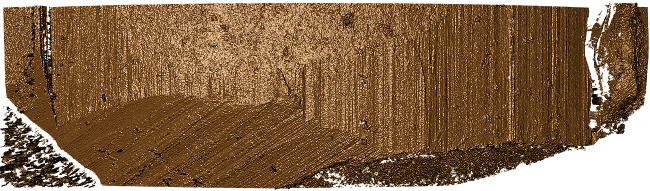
\includegraphics[width=0.475\linewidth]{./images/B1-B1-L6} }
\subfloat[Br2-B2-L5 (tank rash)\label{fig:tankrash2}]{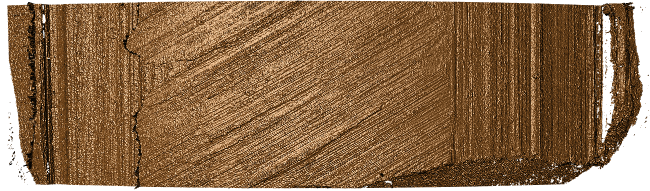
\includegraphics[width=0.475\linewidth]{./images/B2-B2-L5} }\newline
\subfloat[Br3-B1-L5 (tank rash)\label{fig:tankrash3}]{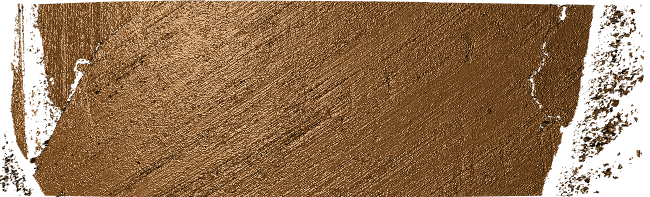
\includegraphics[width=0.475\linewidth]{./images/B3-B1-L5} }
\subfloat[Br8-B1-L6 (tank rash)\label{fig:tankrash4}]{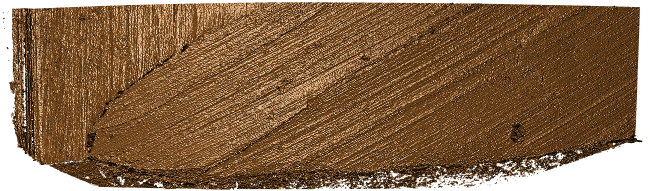
\includegraphics[width=0.475\linewidth]{./images/B8-B1-L6} }\newline
\subfloat[Br8-B2-L2 (pitting)\label{fig:tankrash5}]{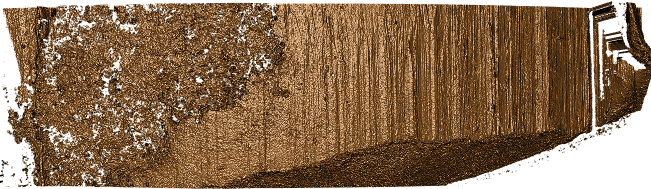
\includegraphics[width=0.475\linewidth]{./images/B8-B2-L2} }
\subfloat[Br8-B2-L6 (tank rash)\label{fig:tankrash6}]{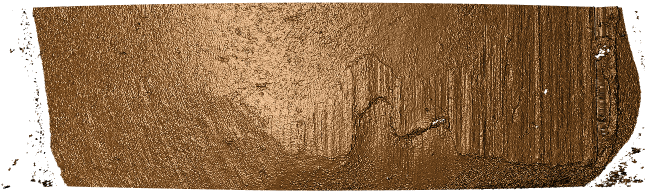
\includegraphics[width=0.475\linewidth]{./images/B8-B2-L6} }\newline
\subfloat[Unk-E-L6 (tank rash)\label{fig:tankrash7}]{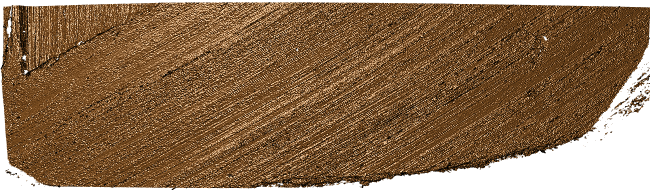
\includegraphics[width=0.475\linewidth]{./images/NA-BE-L6} }
\subfloat[Unk-I-L6 (tank rash and break-off)\label{fig:tankrash8}]{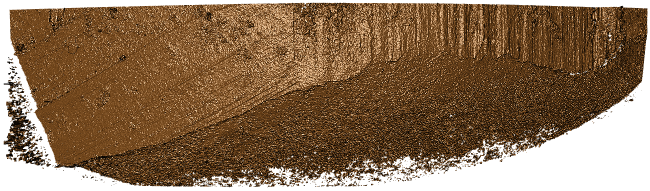
\includegraphics[width=0.475\linewidth]{./images/NA-BI-L6} }\caption[Overview of bullet lands with prominent deficiency such as tank rash or extreme pitting in the Hamby-44 study]{Overview of bullet lands with prominent deficiency such as tank rash or extreme pitting in the Hamby-44 study.}\label{fig:tankrash}
\end{figure}


\end{knitrout}

Three lands from bullets known to be fired from barrel 8 are affected, producing low scores for barrel 8 in \autoref{fig:h44}. We also see that questioned bullet 'I' is affected, explaining some of the low similarity scores for this bullet.
None of the lands of any of the bullets in the other studies are affected by tank rash in a similar manner.










\begin{knitrout}
\definecolor{shadecolor}{rgb}{0.969, 0.969, 0.969}\color{fgcolor}\begin{figure}

{\centering \includegraphics[width=\textwidth]{figures/compare-land-to-land-1} 

}

\caption[Density curves of land-to-land similarity scores from RF scores (top), cross-correlation (middle), and consecutive matching striae (CMS)(bottom)]{Density curves of land-to-land similarity scores from RF scores (top), cross-correlation (middle), and consecutive matching striae (CMS)(bottom). Different colors indicate same source versus different source for each land. RF scores for different source comparisons are generally well below 0.5. Some same-source comparisons are also below 0.5 for RF scores, indicating potential problems with at least one of the lands involved in the comparison.}\label{fig:compare-land-to-land}
\end{figure}


\end{knitrout}

When evaluating classifier performance, it is common to use a receiver operating characteristic (ROC) curve, which plots the percent of wrong identifications against the percent correct identifications for each possible value of the cutoff between the two classes (in this case, known match and known non-match). As the land-to-land scores are not perfectly separated, we can use ROC curves to distinguish between the performance of the different methods and studies. The ROC curves for the land-to-land scores are shown in \autoref{fig:roc-auc} (a). A perfect classifier would have 100\% correct identifications and 0\% wrong identifications, e.g. the ROC curve would be a right angle at $(0, 100)$. Classifiers with better performance will be closer to this corner of the plot. A random classifier would have an ROC curve that was a straight diagonal line through $(0,0)$ and $(100,100)$.










\begin{knitrout}
\definecolor{shadecolor}{rgb}{0.969, 0.969, 0.969}\color{fgcolor}\begin{figure}

{\centering \subfloat[ROC curves\label{fig:roc-auc1}]{\includegraphics[width=0.51\textwidth,height=0.63\textwidth]{figures/roc-auc-1} }
\subfloat[Area under the curve (AUC)\label{fig:roc-auc2}]{\includegraphics[width=.4725\textwidth,height=0.63\textwidth]{figures/roc-auc-2} }

}

\caption[ROC curves and AUC for each (set) of the studies for the random forest score (RF), cross correlation (CC) and consecutively matching striae (CMS)]{ROC curves and AUC for each (set) of the studies for the random forest score (RF), cross correlation (CC) and consecutively matching striae (CMS).   As seen in the ROC curves, the algorithm performs the least well on set 2 of the Houston FSI study. Based on AUC, the overall performance on all sets is very good to excellent for both the cross correlation and the random forest score, and moderate for CMS scores. At the land level there is no significant difference in prediction power between RF score and cross correlation.}\label{fig:roc-auc}
\end{figure}


\end{knitrout}

In \autoref{fig:roc-auc}a, the Houston FSI G1 and G3 curves and the Phoenix PD curve show excellent performance; Houston FSI G2 and Hamby 44 show still a very  good performance. Area under the curve (AUC) values, which summarize ROC curves, are shown in \autoref{fig:roc-auc}b. AUC values are useful for differentiating between poor, good, and excellent model performance, but are not particularly useful when determining which of several models with approximately the same level of performance should be used \citep{marzban_roc_2004}. %Hamby 44 and Phoenix PD are the only studies with a somewhat noticeable difference between the AUC score for RF compared to cross correlation, but even those differences are not statistically significant.

\autoref{fig:eer} shows an overview of Equal Error and their thresholds based on the ROC curves of \autoref{fig:roc-auc}. Equal error rates are the error rates when the sensitivity and specificity of a test are equal, i.e.\ we see the same percentage of missed and wrong identifications for a land-to-land comparison. Equal errors based on CMS of two lands are significantly higher than equal errors based on cross correlation or the RF score. At best, RF score and cross correlation have an equal error of around 5\% for land-to-land comparisons. 
% Interestingly, for consecutively matching striae, equal errors are reached for just two matching striae, which from a practical point of view is not sustainable. A  CMS of 6 or above is an established cutoff used in identifications; when applied to the land-to-land comparisons, it is much more likely to result in a missed identification than a wrong identification. A threshold of 6 leads to 21 wrong identifications out of 49,286 different-source comparisons (0.04\% errors, or about 4 errors for each 10,000 evaluations); when applied to same-source comparisons, 517 of 715 same-source lands were incorrectly classified as exclusions, for an error rate of 80.6\%. 



\begin{knitrout}
\definecolor{shadecolor}{rgb}{0.969, 0.969, 0.969}\color{fgcolor}\begin{figure}

{\centering \includegraphics[width=\textwidth]{figures/eer-1} 

}

\caption[Equal error (in Percent)  and corresponding thresholds for all measures (random forest score, cross correlation and CMS) under all five (sub-)studies]{Equal error (in Percent)  and corresponding thresholds for all measures (random forest score, cross correlation and CMS) under all five (sub-)studies. CMS has an equal error threshold of 2 for all studies, and perform signifcantly worse than both cross correlation and the random forest score. At best, Cross correlation and RF score have equal errors for land-to-land comparisons of around 5\%. The performance of the random forest score is slightly better than the cross-correlation on sets which have higher equal error rates (Houston FSI G2, Hamby 44).}\label{fig:eer}
\end{figure}


\end{knitrout}


\section{Discussion and Conclusions}


At the beginning of this study, we anticipated Hamby 44 would be the easiest set to evaluate because of its similarity to the sets used to train the random forest algorithm. In a surprise turn of events, it was the hardest, in part because of damage to the bullets that obscured LEA striae. It has been shown \citet{lpr2} that parts of lands can be used for successful identifications, if at least 50\% of the land is present (using full-length scores as the reference distribution). The random forest algorithm proposed in \citet{aoas2} is not capable of automatically detecting parts of lands with well-expressed striae. It may be useful to couple the \citet{aoas2} algorithm with an algorithm which assesses the quality of the input data and determines which portions of the data to use for comparison. This would emulate the process used by examiners, who first assess the quality of the evidence and whether there is enough information present to attempt a comparison. One major disadvantage of an automated algorithm is that all of the decisions humans make (recognizing degraded land areas, excluding those areas from consideration, matching only the remaining areas) must be explicitly characterized; however, this explicit characterization means that the process can be scientifically validated to a much higher degree than the human perceptual process. 

All of the studies presented here involve the same type of firearm. We see some variations in scores across different models of Rugers, and it is probable that we will see even bigger variations with different brands of firearms that vary in number of lands and land length. We also know that different firearms and ammunition combinations mark differently well \citep{boltonkingPreventingMiscarriagesJustice2016, bonfantiInfluenc1999}. Rugers are among the firearms that mark very well, so we would correspondingly expect to see lowered similarity scores for other firearms. While the performance of cross-correlation and random forest scores are similar when evaluated on Rugers, it is likely that the additional information used to generate the random forest score may be useful when comparing bullets from barrels which produce fewer distinctive marks. A future study will compare the performance of the random forest score, cross-correlation score, and CMS on non-Ruger barrels. The random forest algorithm is trained on scans taken at the land level, so barrels with polygonal rifling, such as Glocks, which do not introduce well defined lands on bullets, cannot be compared using the random forest algorithm examined here. In addition, we plan to re-fit the random forest using a wider set of scans taken at different resolutions, with different ammunition, fired from barrels of different models. We expect that a random forest trained on a wider set of input data will be more likely to produce scores which meet the criteria for monotonicity and stability. 

The random forest matching algorithm presented in \citet{aoas2} does perform well on three different external test sets. While a single cutoff value cannot be used to distinguish matches and non-matches across the different test sets, the algorithm makes no errors when a set-specific cutoff value is used on bullet-to-bullet scores aggregated using sequence average maximum. This performance is on par with the performance of forensic examiners. For a future round of the Houston study, we are planning to compare the algorithmic performance directly with scores given by forensic toolmark examiners. The algorithm's score is not intended to replace an examiner's judgment; instead, it provides a complementary tool to measure, quantify, and compare the similarity of two bullets in an identification. With more research into the behavior of score-based likelihood ratios, the random forest score may also be used to compute a SLR to explicitly quantify the strength of the match between two bullets relative to other matches in the population.
By validating the algorithm on external test sets, we have demonstrated that the method can be generalized to different types of ammunition and is not overly sensitive to small differences in rifling procedure. Future studies can and should generalize this to a wider range of external test sets to establish the limits of the algorithm's generalizability.



\section{References}

\bibliography{bibfile}

\end{document}

% <!--include marginal distributions of training data and compare to test data-->


